
\chapter{Methodology and implementation}

\todo[inline]{Description of experiments, model architecture and reasoning behind choices. Not yet enough equations but I'm not sure how much should be included. }

\section{Dataset}

As previously mentioned, we use a dataset that represents two modalities. 

The Open Images dataset collated by Google\cite{openimages}  consists of 7337077 annotated images tagged with concepts that occur within them. Images and concepts are given IDs, and the number of occurrences of a particular concept ID in a particular image with a specific ID are recorded. We use this co-occurrence data to build a co-occurrence matrix that indicates which concepts occur together in the dataset. This is exactly analogous to the co-occurrence matrix used in \cite{pennington2014glove} from which GloVe embeddings are derived. (The dataset also contains other annotations like bounding boxes, but these are not used in this experiment)

The AudioSet dataset \cite{audioset} consists of 22160 annotated sound clips, where clips are given IDs and labelled according to which concept IDs are present in them. As this dataset is also collated by Google, the label IDs are almost the same (a small amount of preprocessing had to be done to exactly match them). Similarly to the above, a co-occurrence matrix is created from the annotation data. 

In total there are 20522 labelled concepts; 19996 from Open Images and 526 from AudioSet, with an intersection of 230 concepts present in both datasets. 

The concept labellings are both human- and machine-generated. They are not always completely accurate. For example, the image below has been labelled, by a human annotator, with the terms ``Tortoise" and ``Sea turtle". As these two terms represent distinct species, the tagged object cannot be both. In the case of this image it is presumably because the image is of a woman sitting next to a fountain in which there is a statue of a tortoise-like animal, the type of which the human tagger could not determine exactly. This pattern persists throughout the image library, where images are tagged with labels that are clearly related, but not always accurate. (In particular the Tortoise / Sea turtle mislabelling appears many times). For the purposes of this study this is less significant, but if we were trying to relate the relationships found by the experiments back to real-life data, it might be. However, the co-occurrence statistics do capture the relationships that humans think exist, even if these are inaccurate. It is a philosophical point as to whether these are accurate in a different way- that of capturing the human judgement of these relationships, even if that judgement is factually incorrect.   

In this experiment, the concept labellings have no connection to other items in the external world. In fact, the embeddings are learnt completely independently of any labellings; the embeddings are numbered by the index they occur in the co-occurrence data. For example, the first index in the Open Images co-occurrence matrix is for ``Sprenger's tulip", a type of flower, which has label ``/m/0100nhbf", but neither of these labels (the human name or the machine ID) are used anywhere in the learning system. Any ``meanings" that we ascribe to relationships between embeddings must be inferred from later re-mapping the names/IDs back to the indexes. If the system learns a system of embeddings that relate concepts 15268 and 5296 in such a way that they are close in embedding space, we will not know until later that the concepts 15268 and 5296 are ``Coffee" and ``Tea" (in which case they are related, and our algorithm is fit for purpose), or that they are ``Sprenger's tulip" and ``Ferret" (in which case they are not related). 

\begin{figure}[H]
    \centering
    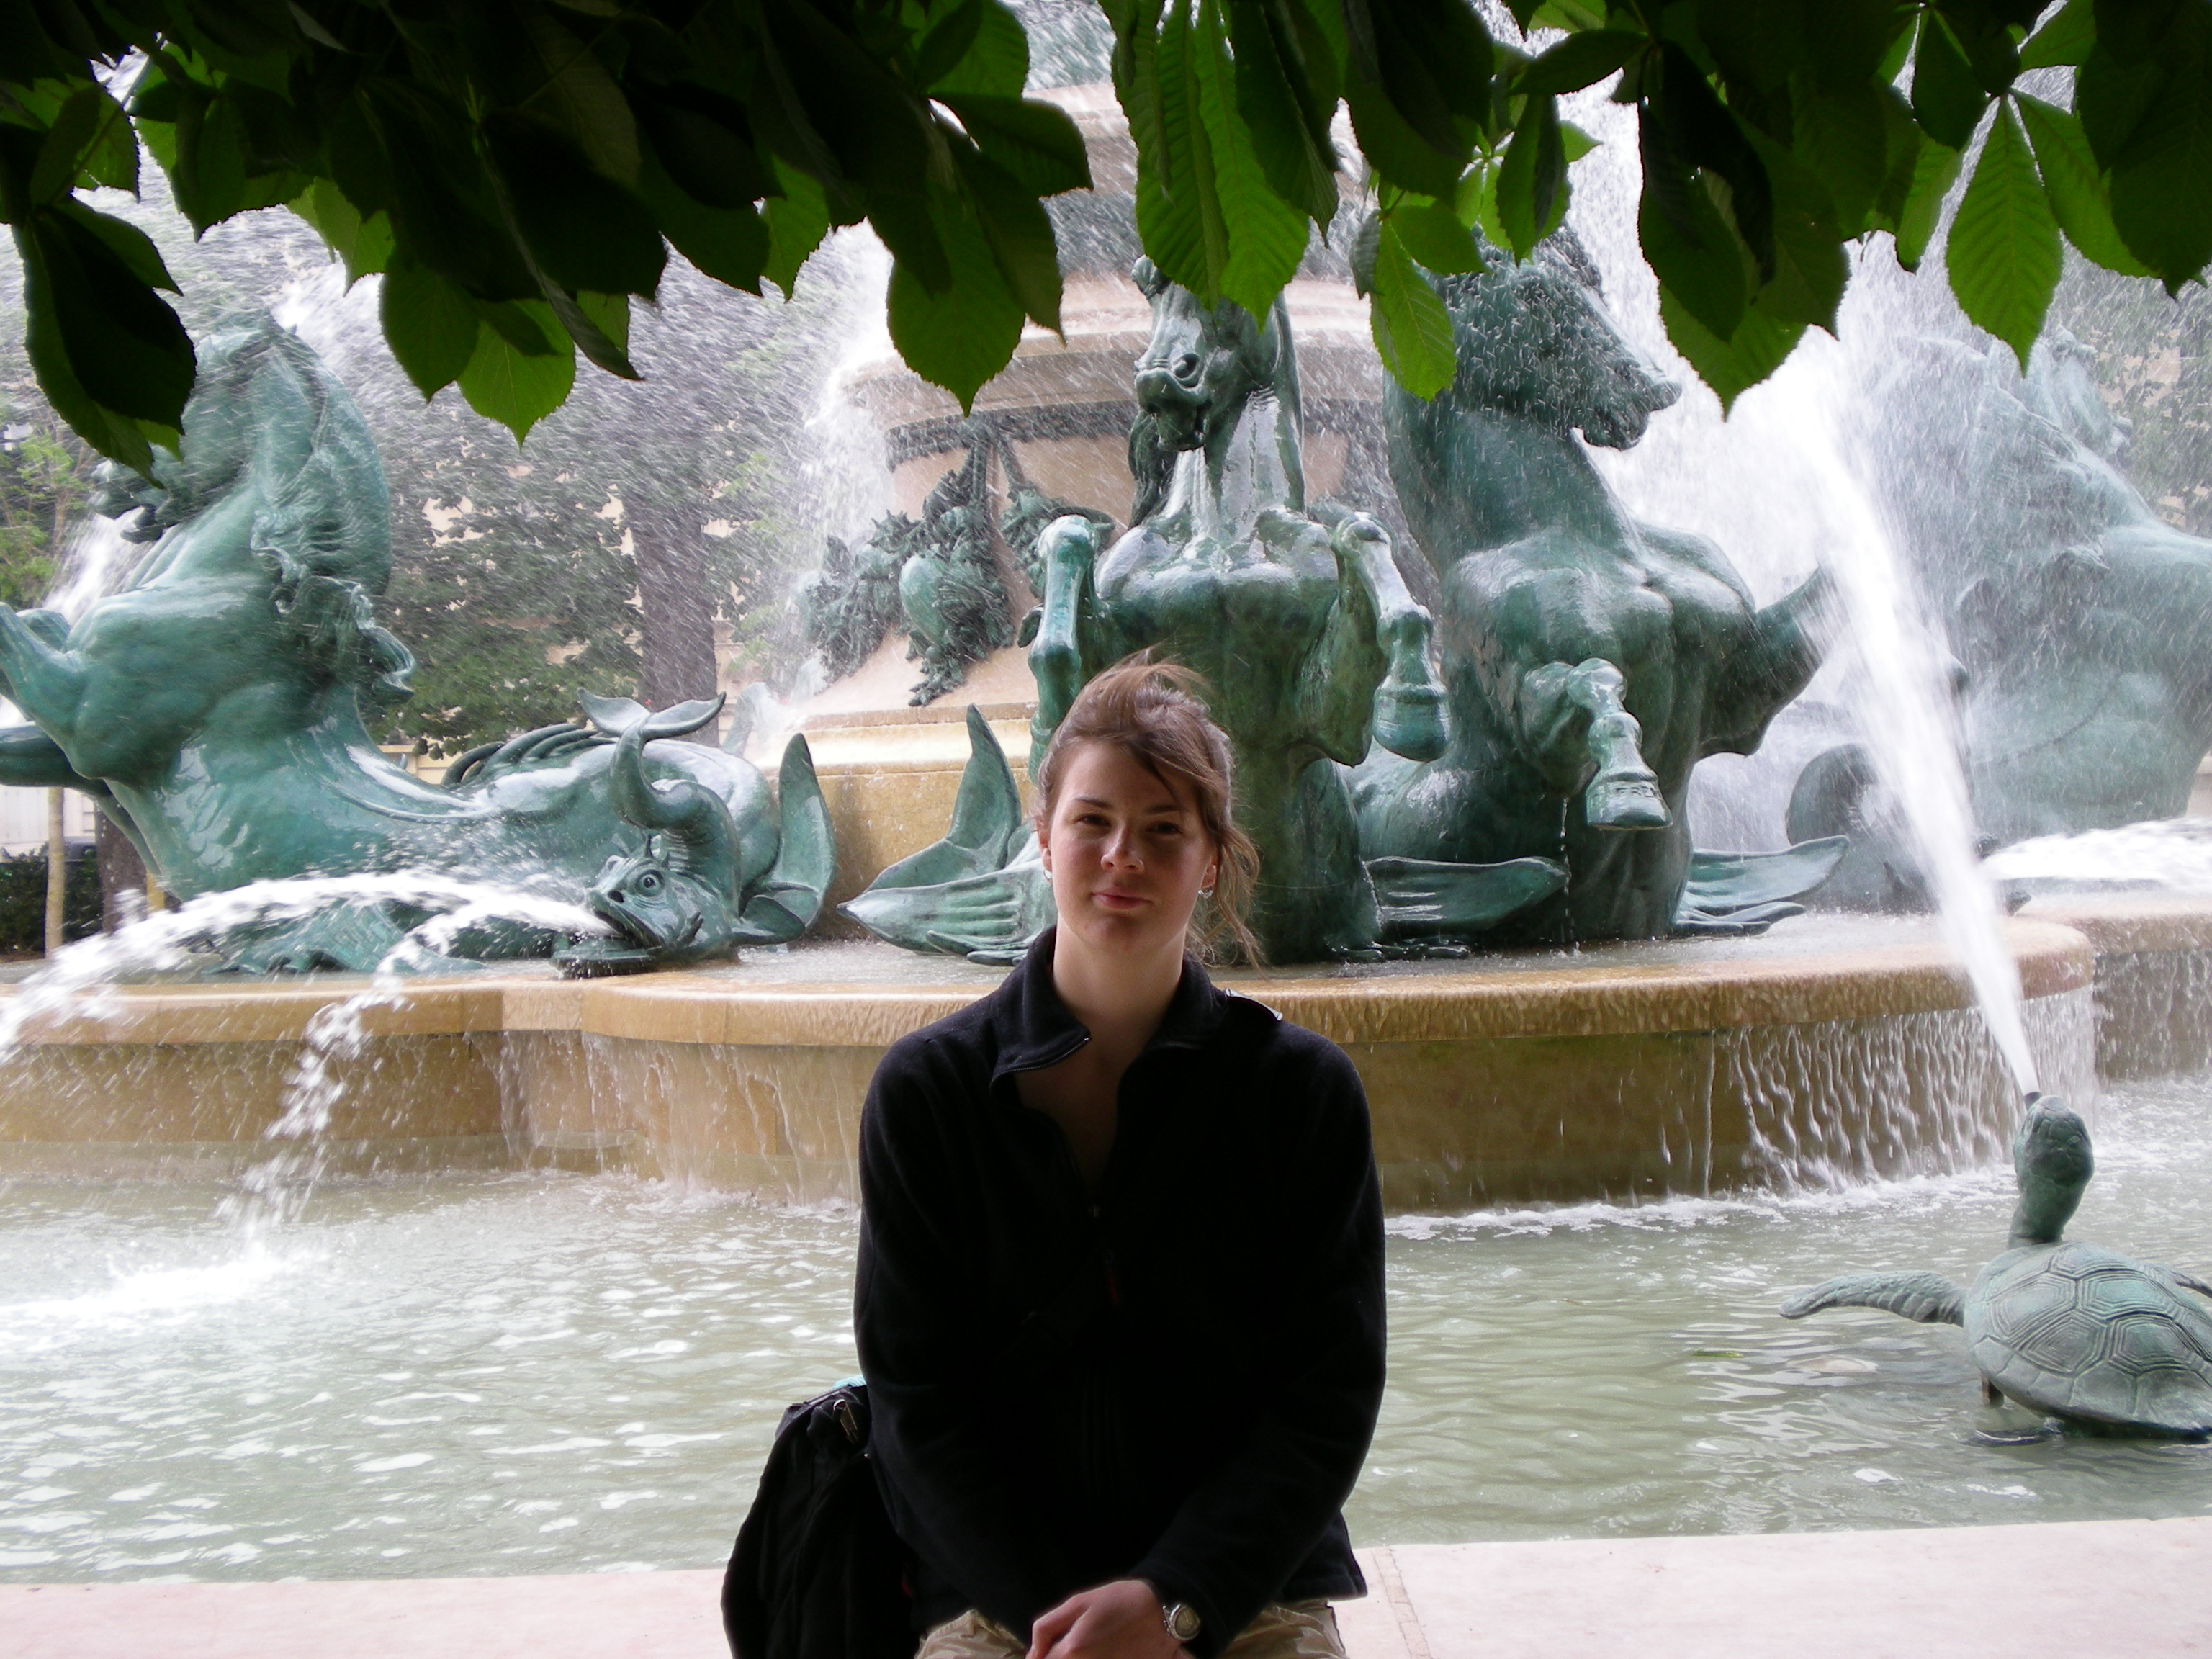
\includegraphics[width=0.95\textwidth]{images/method/tortoise_seaturtle.jpg}
    \caption{
        An image with at least one mislabelled concept: The fountain statue is labelled as both ``Tortoise" and ``Sea turtle"; it cannot be both. 
    }
\end{figure}


The co-occurrence matrices for the Open Images and AudioSet datasets, as well as the concept name to label mapping files, make up the dataset for these experiments. This dataset should represent the statistical distribution of co-occurrence of concepts in the two modalities (image and audio). \\

Other points

\begin{itemize}
    \item Both datasets also have ontology / hierarchy information
    \item Open Images: https://storage.googleapis.com/openimages/2018\_04/bbox\_labels\_600\_hierarchy\_visualizer/circle.html
    \item AudioSet: http://research.google.com/audioset/ontology/index.html
    \item Add item about how co-occurrence matrices were created and saved
\end{itemize}

\section{Choice of embeddings: Probabilistic GloVe embeddings}

As the dataset comprises co-occurrence statistics, it is similar input to that used to learn GloVe embeddings \cite{pennington2014glove}. The GloVe learning algorithm is particularly efficient, as it uses only the non-zero items in the co-occurrence matrix, which for our dataset is extremely sparse. The computational complexity of the model depends on the number of such non-zero items rather than on the size of the co-occurrence matrix. It has been found to produce reasonable clusters of concepts, that is, the concepts learnt from this algorithm are close in embedding space if they are close in semantic space. \cite{pennington2014glove} found that the embedding space produced by this algorithm gave an accuracy of 75\% on a word analogy test, which was state-of-the-art at the time of their publication. GloVe embeddings are also stable, by the metric used in \cite{WordEmbeddingStability}- the amount of overlap between nearest neighbours of an embedding for different runs. As the GloVe embedding is trained by stochastic gradient descent, the embeddings resulting from different random seeds will be different.

We make two further additions to this embedding model. Firstly, we implement probabilistic embeddings; the original GloVe embeddings are deterministic. The probabilistic/deterministic distinction refers not to the learning algorithm (which has a probabilistic component as it uses minibatch gradient descent), but to the embedding representation. The original GloVe embeddings are represented by multidimensional vectors; a single vector for each concept. In our implementation, each probabilistic embedding is intended to represent a multivariate Gaussian distribution with independent dimensions (diagonal covariance matrix). 

A probabilistic embedding is a sample from the following distribution:
\begin{equation}
    \mu + \sigma \N(0, 1)
\end{equation}

Both $\mu$ and $\sigma$ are learnt parameters. In practice, $\sigma$ is further parametrised as follows, to enforce positivity:

\begin{equation}
    \sigma = \ln (1 + \exp (\rho))
\end{equation}

Therefore the full equation for a probabilistic embedding is 

\begin{equation}
\label{eq:stochemb}
    \mu + \ln (1 + \exp(\rho)) \cdot \N(0, 1)
\end{equation}

\subsection{Implementation}

A probabilistic version of the GloVe learning algorithm was implemented in Python using the PyTorch \cite{pytorch}, PyTorch Lightning \cite{pytorchlightning} and Pyro \cite{pyro} libraries. Specifically, a custom neural network layer was implemented which took as input a co-occurrence matrix, and learnt probabilistic GloVe embeddings based on iterating over the concepts represented in the matrix. Each mini-batch represented a random sampling of the rows and columns of the co-occurrence matrix, with all rows and columns being used over the course of one training epoch. 

The GloVe loss function is reproduced here:

\begin{equation}
\label{eq:gloveloss}
\begin{split}
L_{glove} &= \sum_i \sum_j f(X_{ij}) (\vecw_i^T \vecw_j + b_i + b_j - \log X_{ij})^2\\
f(x) &= \begin{cases}
(x/x_{max})^{\alpha}\spaced{if} x \le x_{max}\\
1\spaced{otherwise}
\end{cases}
\end{split}
\end{equation}

\begin{itemize}
    \item The values of hyperparameters $\alpha = 0.75$ and $x_{max} = 100$  are set as in the original paper, \cite{pennington2014glove}. 
    \item The $\vecw_i$ and $\vecw_j$ are samples of the current probabilistic embeddings represented by equation \ref{eq:stochemb}. 
    \item The $X_{ij}$ are co-occurrence statistics of the $i$th and $j$th concept
\end{itemize}

The Pyro library provides backpropagation through the random sampling, as described in \cite{deeplearninggoodfellow} (section 20.9). The next section describes how these probabilistic embeddings were verified. 

\subsection{Validation}

The probabilistic embeddings were validated as follows:

\begin{itemize}
    \item Train embeddings learnt from Open Images and AudioSet co-occurrence data. 
    \item Each domain's embeddings are learnt individually without regard for alignment. 
    \item For each run of each domain, the random seed was manually set. 10 seeds were used in total capturing 10 separate embeddings for each domain. 
    \item The following learning parameters were used:
    \begin{itemize}
        \item Embedding dimension of 6. This choice was heuristic: the test implementation of GloVe embeddings implemented in PyTorch had 1 million unique tokens and dimensionality of 300, to keep the same ratio of effective tokens to dimensionality, 6 was the closest integer. 
        \item Mini-batch size of 500
        \item The Adam \cite{kingma2017adam} optimiser, with learning rate 0.01
        \item 250 epochs of training for Open Images and 2000 epochs for AudioSet. This was enough to ensure convergence of the GloVe loss decreasing to asymptotic levels. 
        \begin{itemize}
            \item It is interesting that AudioSet needed many more epochs to converge. This is consistent with an earlier point mentioned in \cite{GOLDSTONE2002295} that systems with more concepts are easier to learn as they are more constrained. 
        \end{itemize}
    \end{itemize}
    \item No hyperparameter tuning was done; as this is not a supervised learning problem, we measure convergence only by the decrease in GloVe loss (equation \ref{eq:gloveloss}). Overfitting does not occur and the GloVe loss decreases steadily to an asymptotic value. 
\end{itemize}

The output of this training are 10 sets of probabilistic embeddings (parametrised by their mean and variance) for each domain (Open Images / AudioSet). These embeddings are doubly stochastic; one source is stochasticity in the learning algorithm leading to 2 runs with different seeds converging to different mean embeddings, and the other is caused by each embedding being a sample from a multivariate Gaussian distribution. 

\subsubsection{Clustering}
As a sanity check, the t-SNE (t-Distributed Stochastic Neighbor Embedding, \cite{tsne}) algorithm was  used to reduce the dimensionality of the embeddings from 6 to 2, and the resulting points plotted for the top 300 most frequently occurring concepts in each domain (measured by number of occurrences in images or audio clips). As we expected, there are clear clusters of concepts visible. This clustering was visible over different seeds. While t-SNE adds a further level of stochasticity during the dimensionality reduction process, two runs of t-SNE on the same input data with the same t-SNE random seed set, will produce the same result. Therefore, we can assume that the stochasticity introduced by t-SNE is accounted for. 

This is a qualitative analysis only intended to confirm that the implementation is correct and converges to embeddings that have sensible semantic relationships. This technique of using t-SNE to sanity check embedding quality is commonly used in other similar experiments (for example \cite{CoocurrenceVisionLanguage2021}). 

\begin{figure}[H]
    \centering
    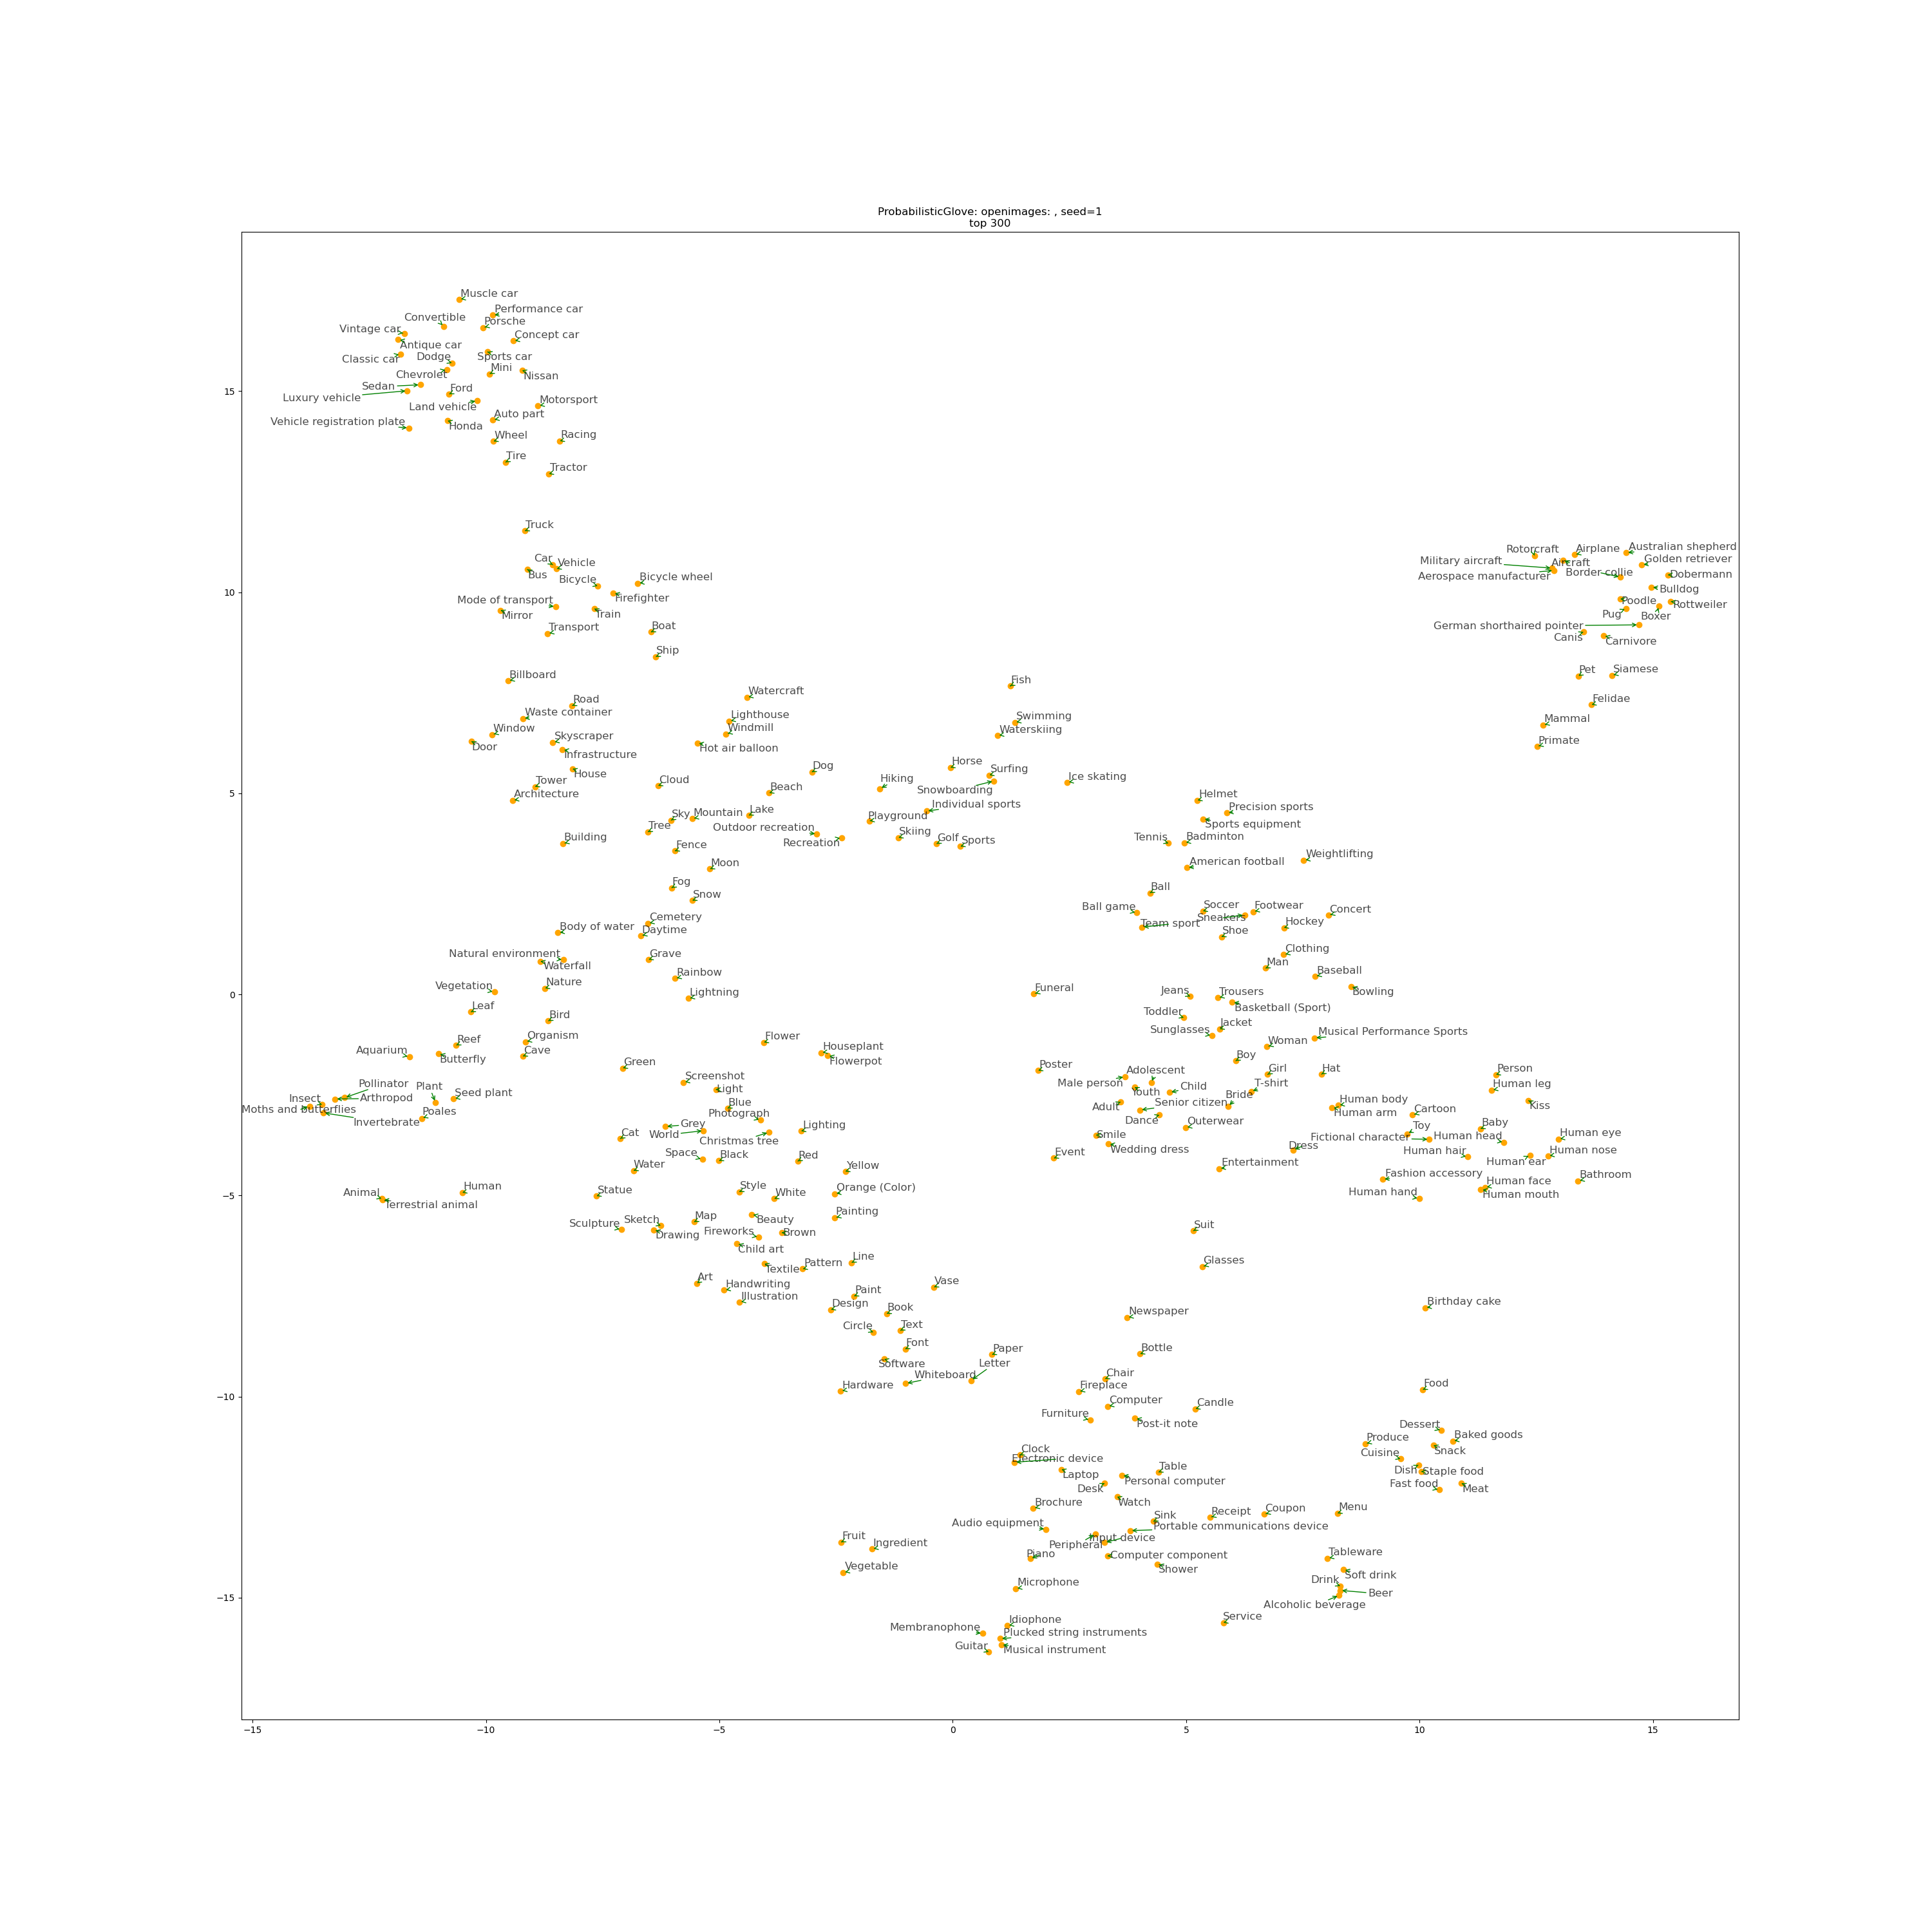
\includegraphics[width=1.0\textwidth]{images/method/probabilistic_independent/top300_tsne_openimages__ProbabilisticGlove_1.png}
    \caption{
        Open Images top 300 most common concepts. There are clearly visible clusters corresponding to, amongst other things, different types of dog, different types of vehicle, and different types of human body part. Blue points correspond to concepts present in both Open Images and AudioSet. Orange points correspond to the top 300 most frequently occurring concepts in the Open Images dataset (that are not also in the intersection of concepts).
    }
    % generated by inspect_results.py 
\end{figure}

\begin{figure}[H]
    \centering
    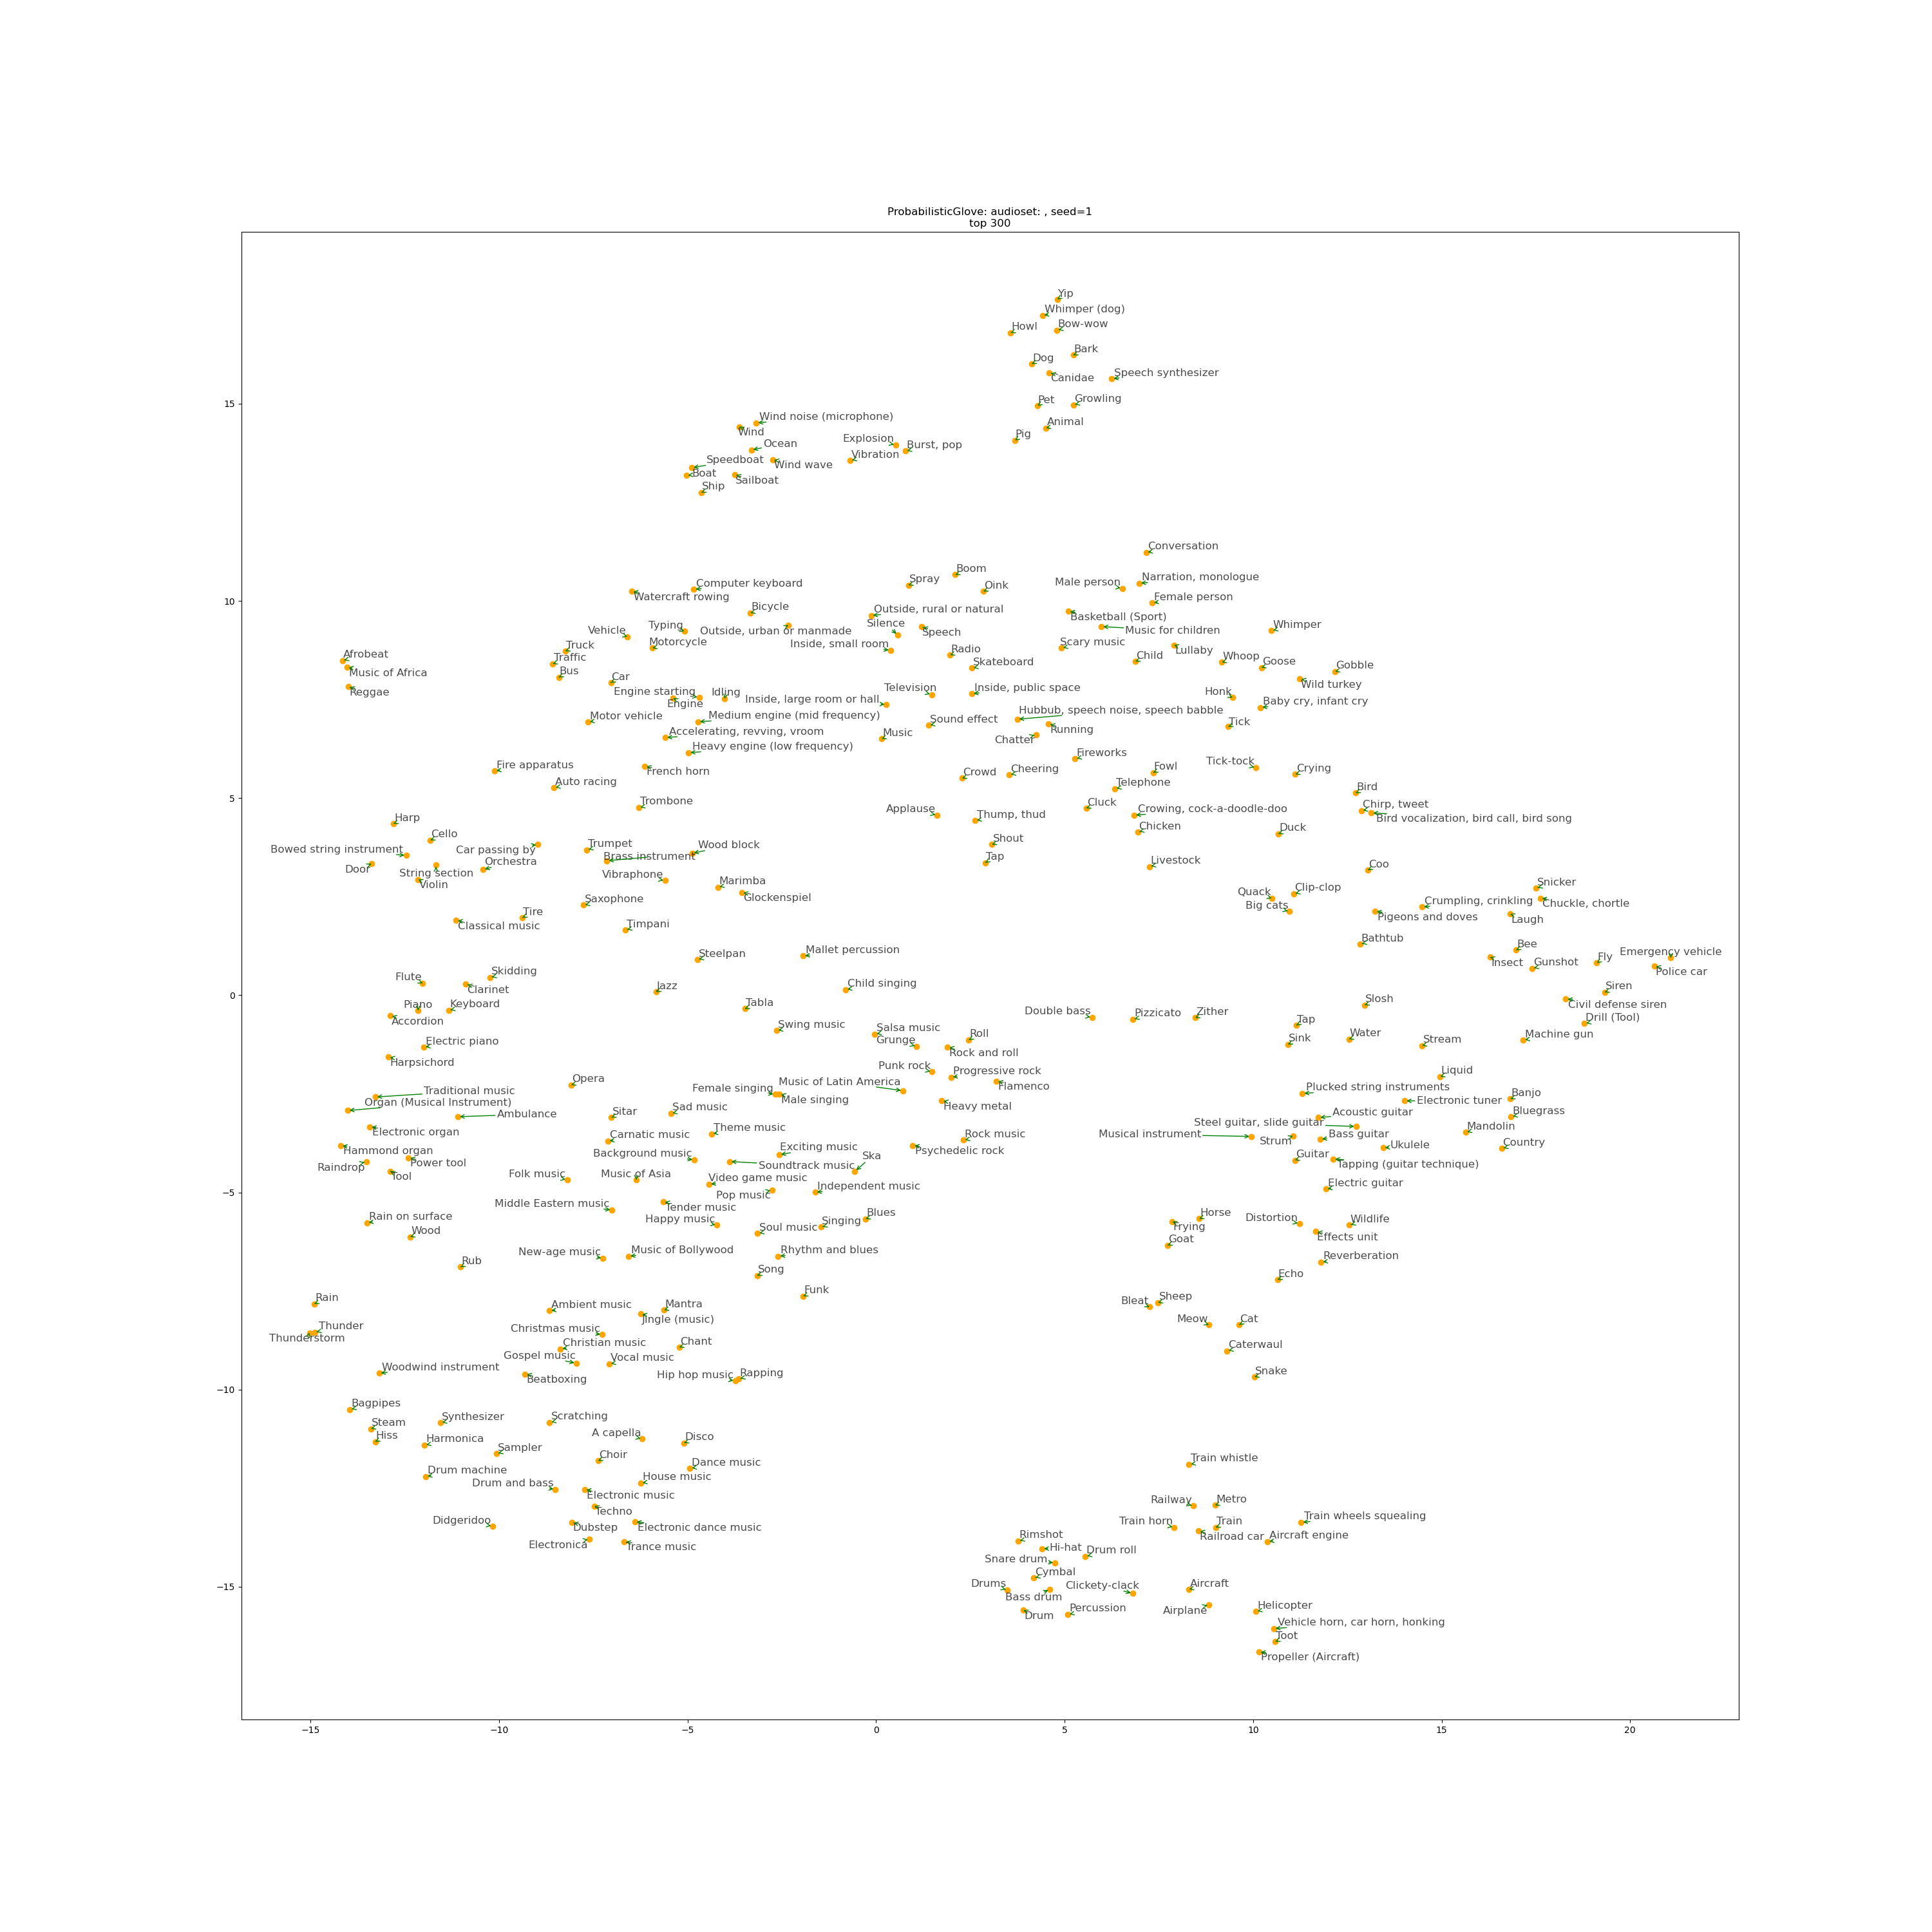
\includegraphics[width=1.0\textwidth]{images/method/probabilistic_independent/top300_tsne_audioset__ProbabilisticGlove_1.png}
    \caption{
        AudioSet top 300 most common concepts. Again there are clearly visible clusters comprising, for example, sounds made by water, sounds made by percussion instruments, and sounds made by dogs. Blue points correspond to concepts present in both Open Images and AudioSet. Orange points correspond to the top 300 most frequently occurring concepts in the AudioSet dataset (that are not also in the intersection of concepts).
    }
    % generated by inspect_results.py 
\end{figure}

Plots of the Open Images top 300 concepts t-SNE plots annotated to show the clusters, for random seeds 1 and 2, show that roughly the same concepts cluster for each run. They also reveal a characteristic of our alignment problem: The cluster arrangements relative to each other across runs are not consistent. Ideally, we would like the different clusters to have the same spatial arrangement across runs. As described in \cite{SHEPARD19701}, we would like to identify second order isomorphisms in the data; not just the clusters, but the relationship between the clusters. 

\begin{figure}[H]
    \centering
    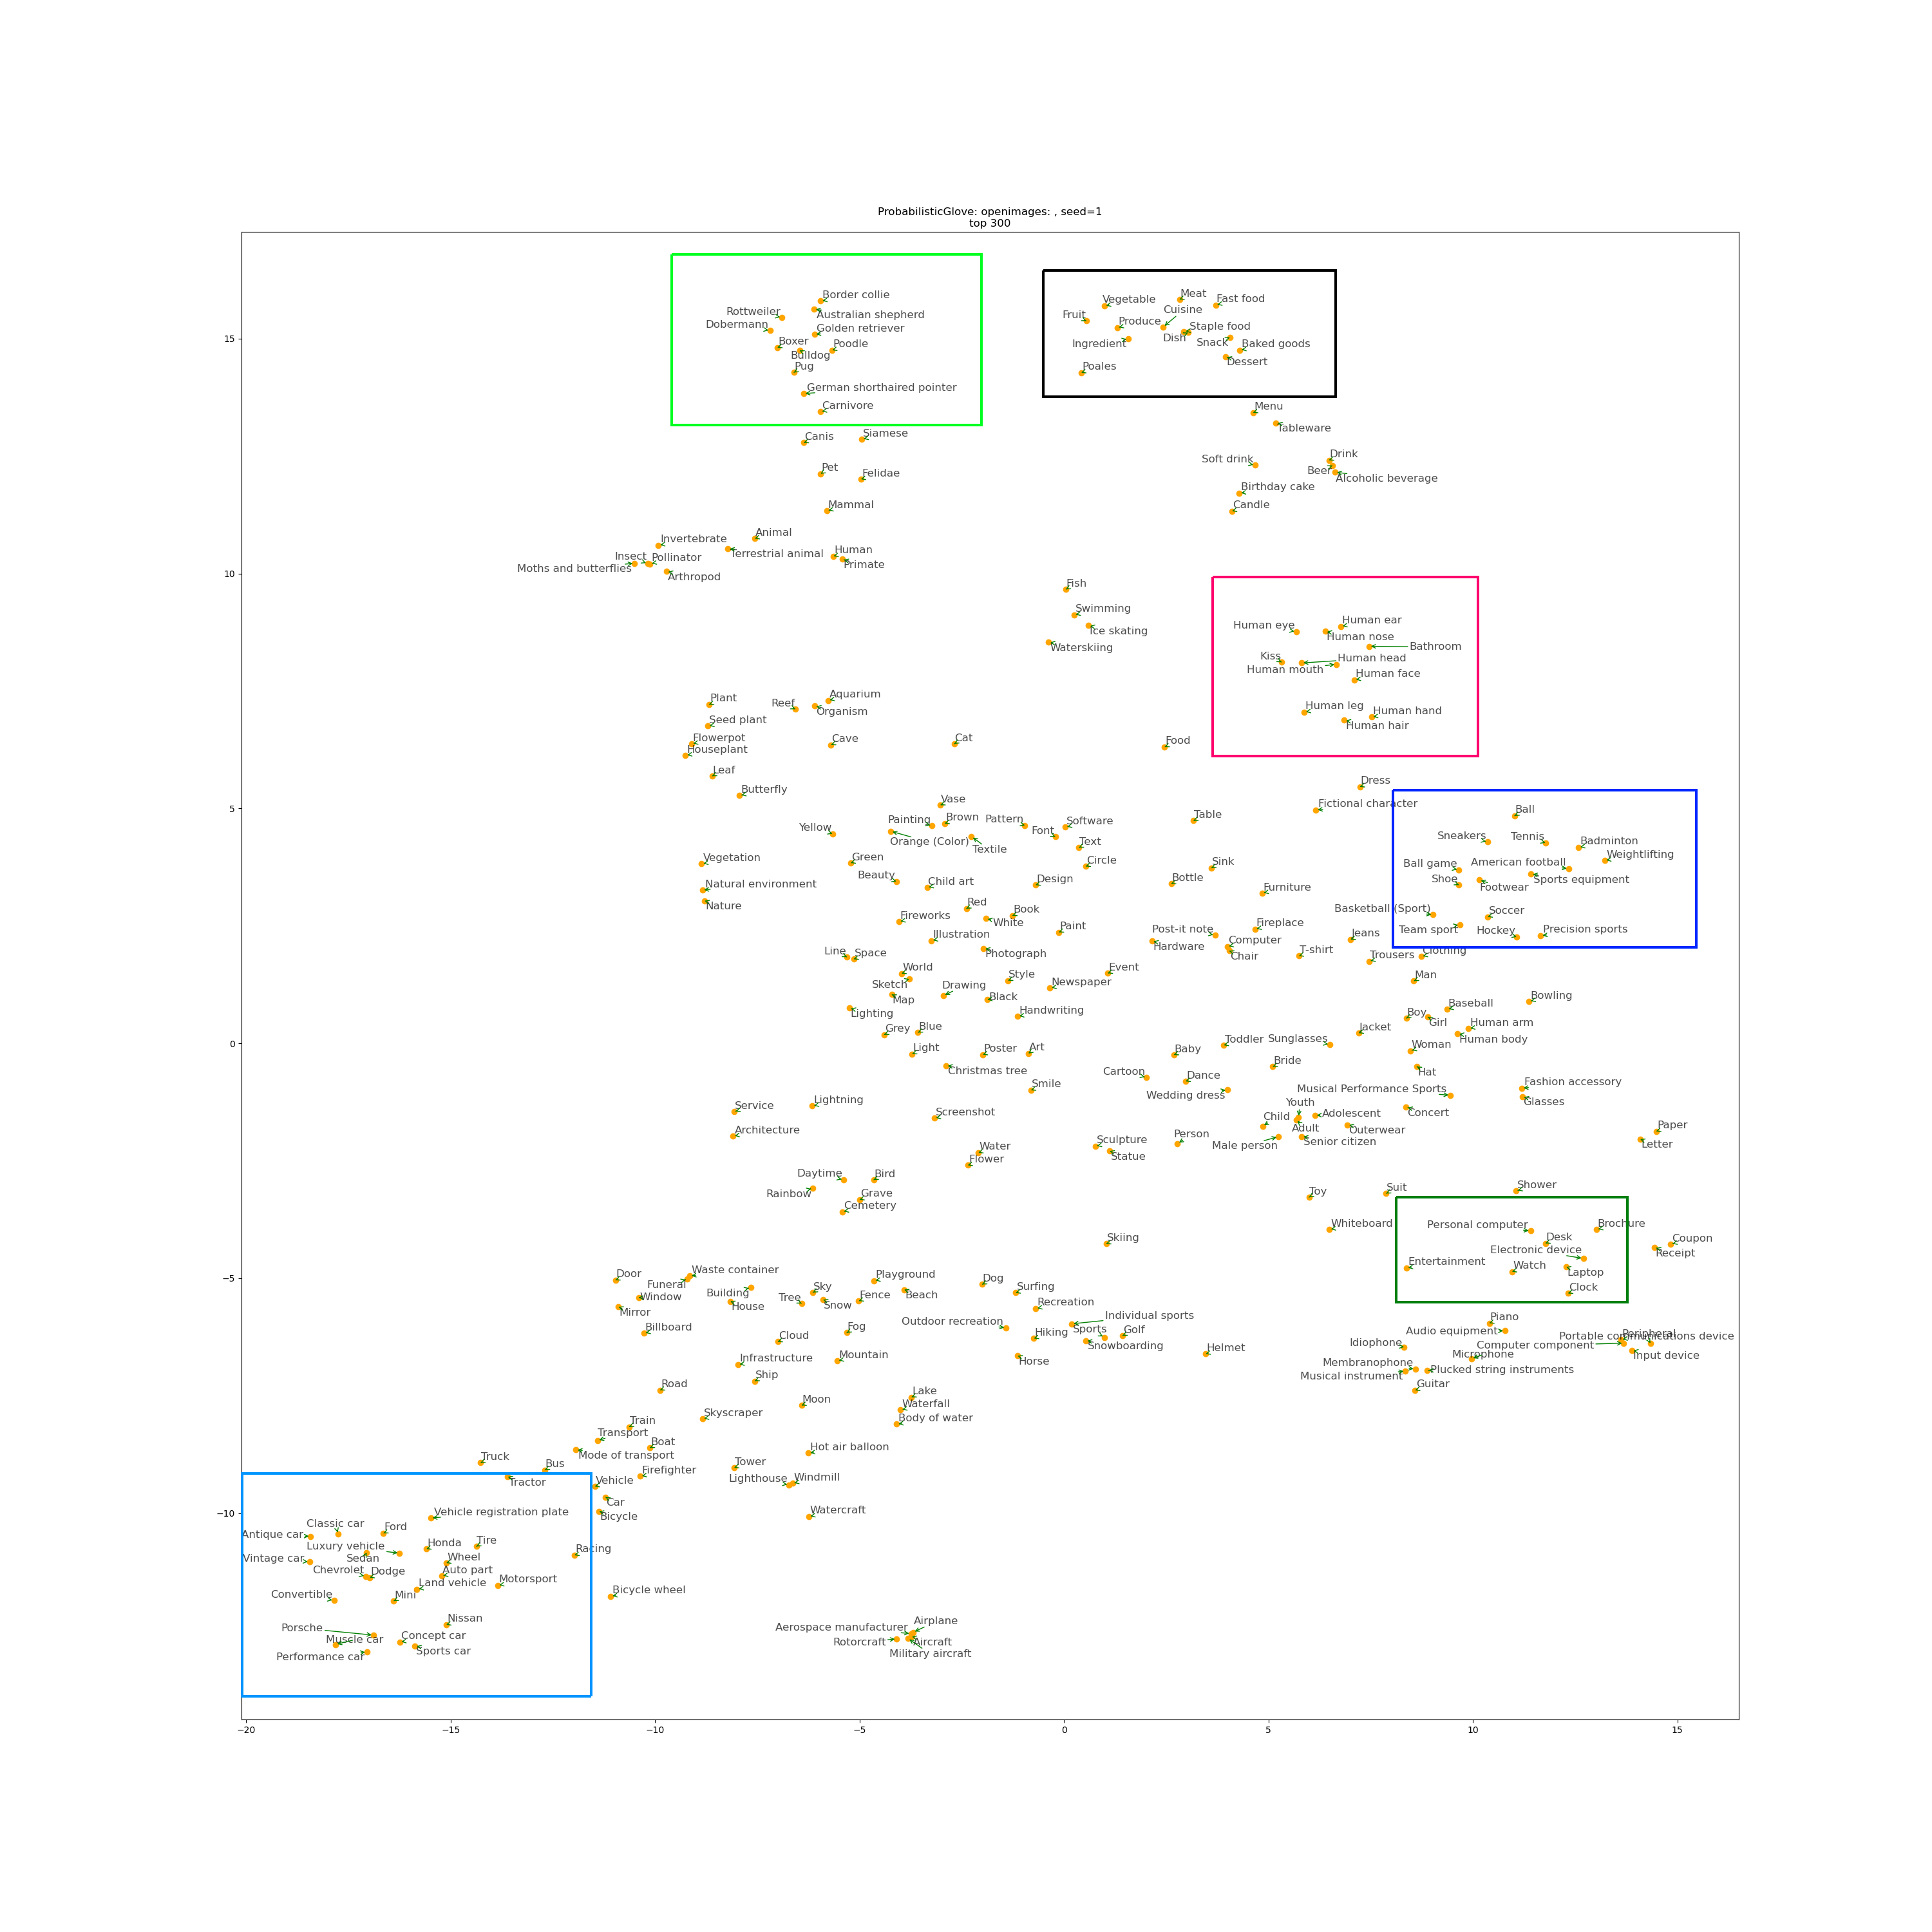
\includegraphics[width=0.95\textwidth]{images/method/probabilistic_independent/top300_tsne_openimages__ProbabilisticGlove_1_clusters.png}
    \caption{
        Coloured boxes indicate clusters 
    }
    % generated by inspect_results.py 
\end{figure}

\begin{figure}[H]
    \centering
    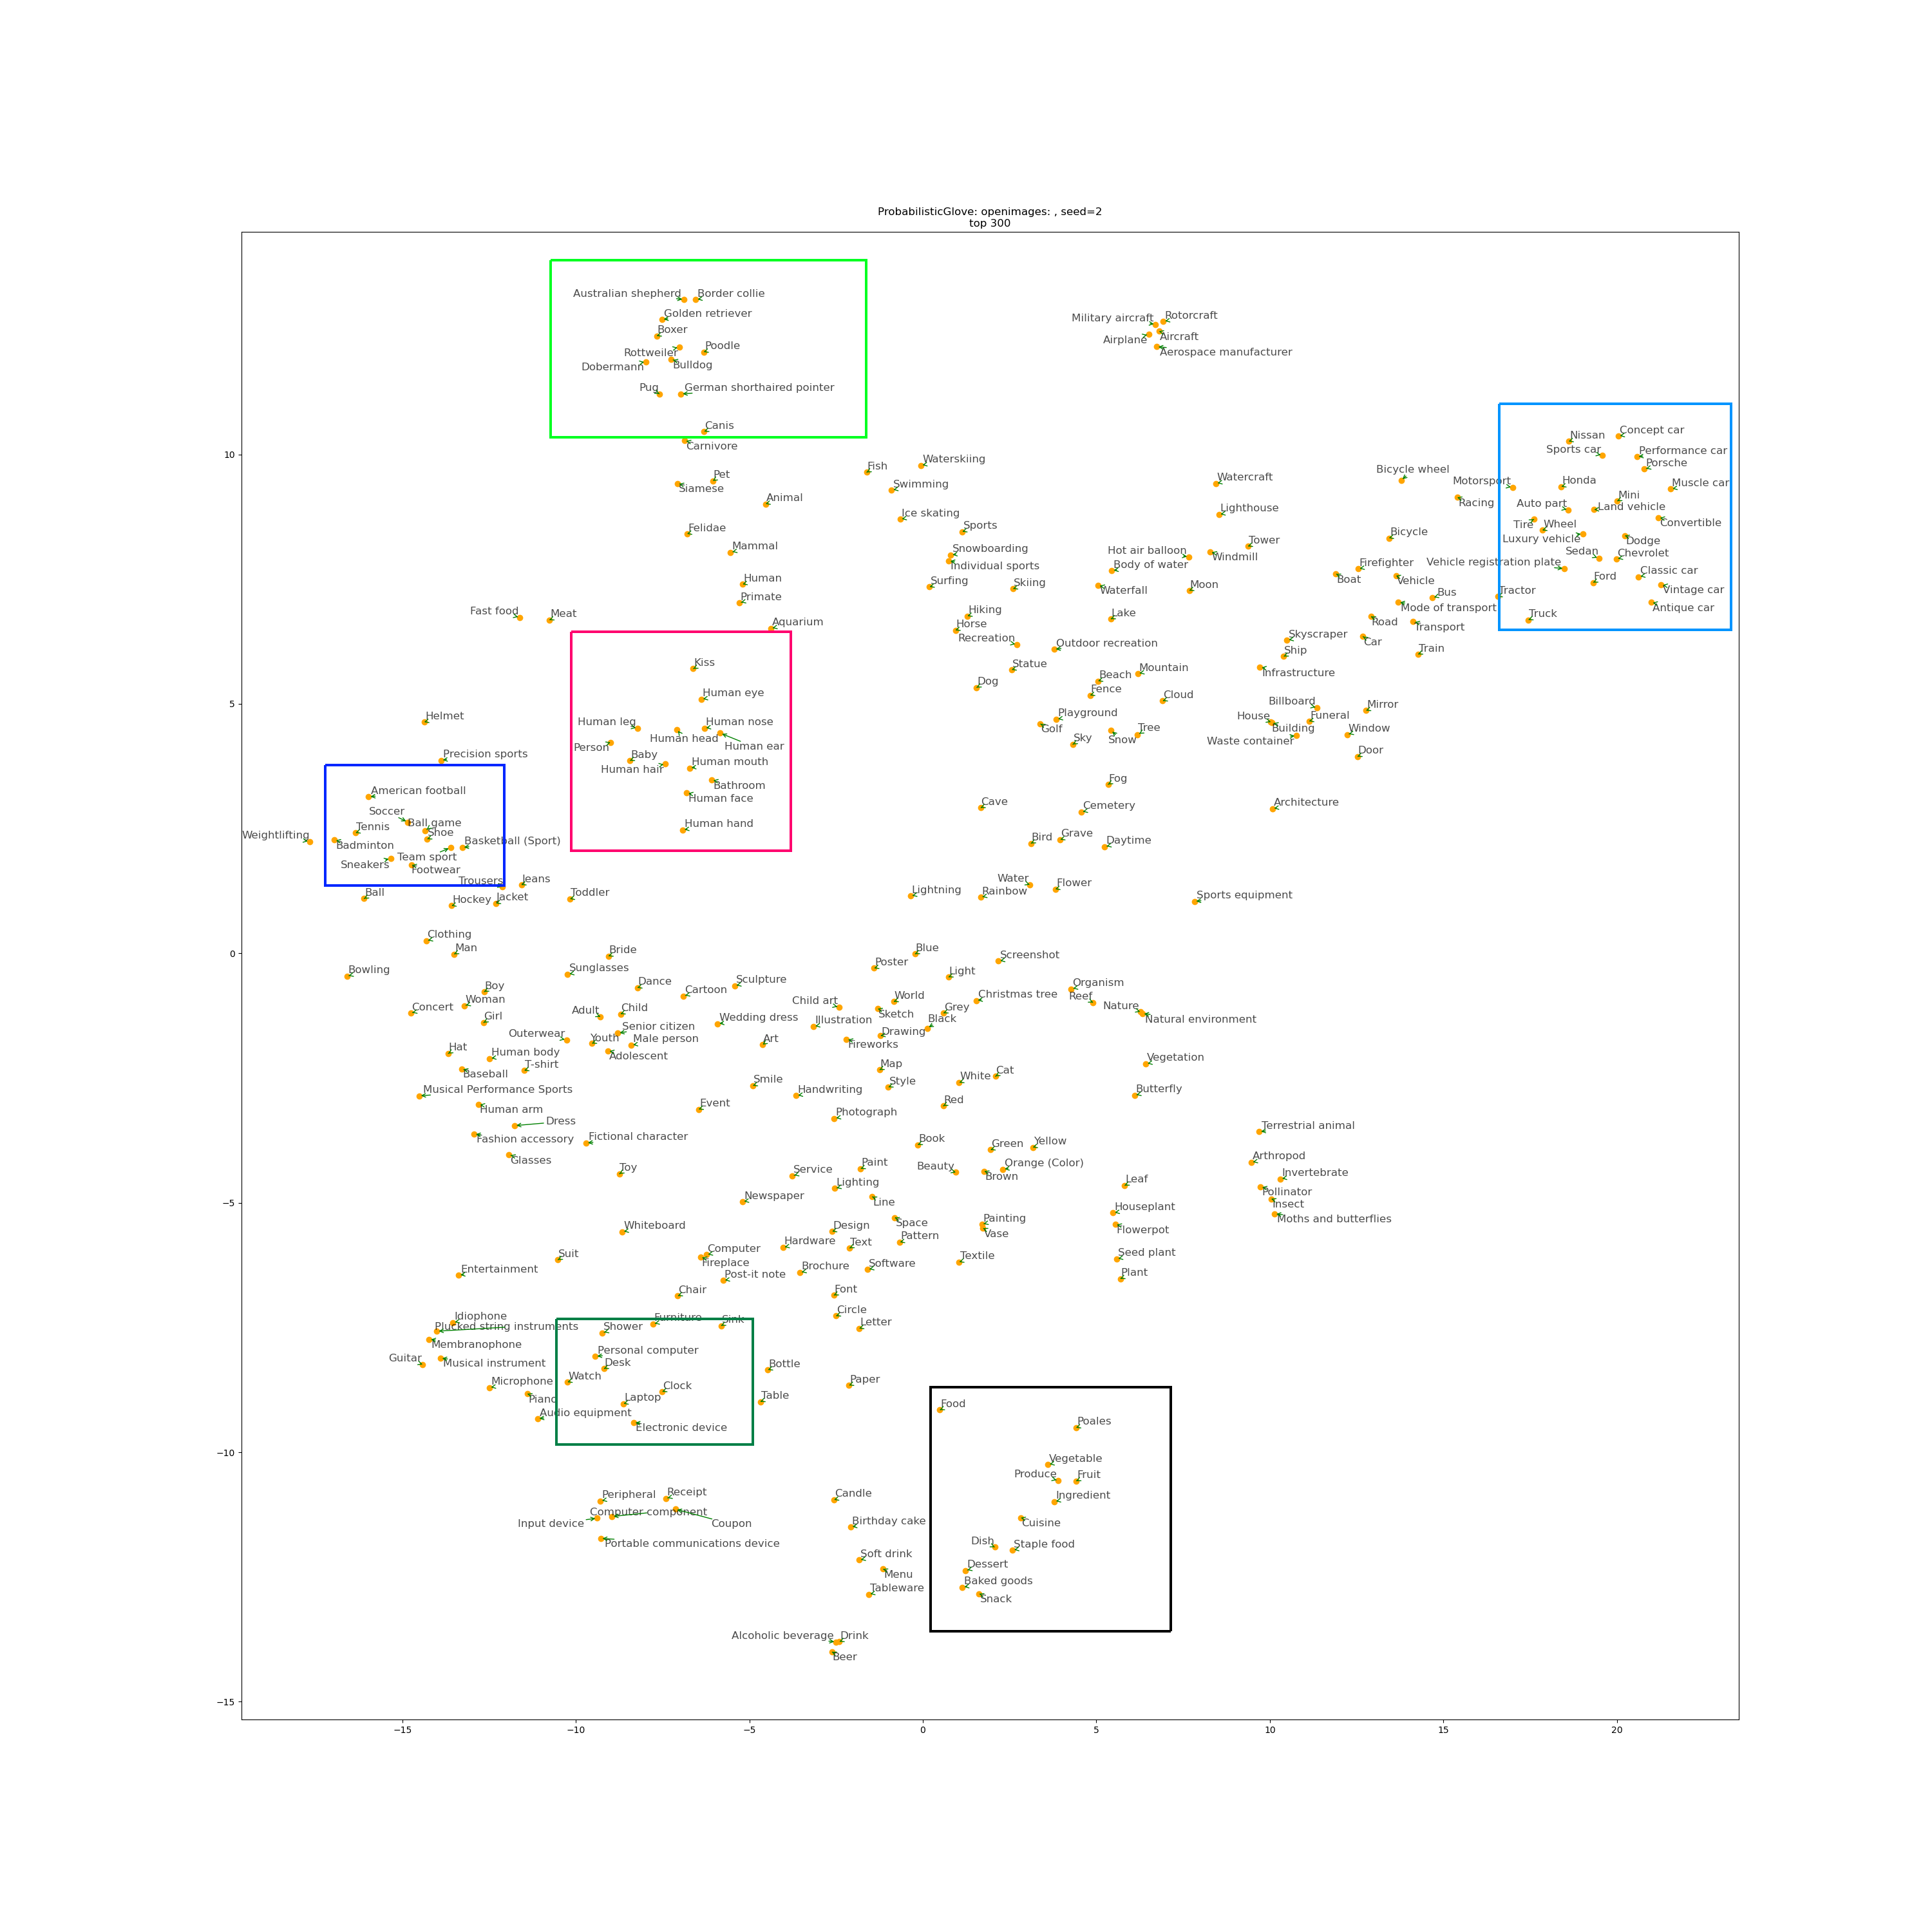
\includegraphics[width=0.95\textwidth]{images/method/probabilistic_independent/top300_tsne_openimages__ProbabilisticGlove_2_clusters.png}
    \caption{
        The same clusters are in different locations in embedding space compared to the previous run, and their orientation relative to each other is different; it is not a simple rotation and stretch of the clusters. Although t-SNE introduces more stochasticity, both t-SNE runs were done with the same t-SNE random seed set, which is known to generate the same output if given the same inputs. 
    }
    % generated by inspect_results.py 
\end{figure}

\subsubsection{Learnt parameters of the probabilistic embeddings}

We also examine the learnt means and variances, $\mu$ and $\sigma = \ln(1 + \exp(\rho))$, of each embedding. 

This is done as follows for each domain (Open Images and AudioSet separately):

\begin{itemize}
    \item Dot product distances are calculated between the learnt $\mu$ (the mean of the stochastic embeddings) for every pair of concepts. Since the stochastic embeddings can be thought of as distributions about a mean, where the mean would be the embedding learnt in the deterministic case. 
    \item This gives a similarity matrix between each embedding and itself, for each seed. 
    \item The correlation between the values of each run's similarity matrix with every other run was computed, and the mean value taken. A high value should indicate that the concepts in each run have the same similarity with each other. 
    \item This was $ \pm $ for AudioSet and $0.9989 \pm 8.5261e-06$ for OpenImages. 
% /home/petra/spond/spond/experimental/glove/results/audioset/ProbabilisticGlove/audioset_analytics.hdf5
% /home/petra/spond/spond/experimental/glove/results/openimages/ProbabilisticGlove/openimages_analytics.hdf5
\end{itemize}

The variances were examined by analysing the entropy of each embedding. Since each embedding is a multivariate Gaussian with a diagonal covariance matrix:

\begin{equation}
\begin{split}
H(x) &= \frac{1}{2} \ln |\Sigma| + \frac{D}{2}(1 + \ln(2 \pi))\\
&= \frac{1}{2} \ln \prod_{i=1}^D \sigma_i + \frac{D}{2}(1 + \ln(2 \pi))\\
\end{split}
\end{equation}

In the above, $\sigma_i$ is the variance for dimension $i$. 
 
By examining histograms of the entropies of each run (with different seeds), we can check if the algorithm is producing stable results. 
\begin{figure}[H]
    \centering
    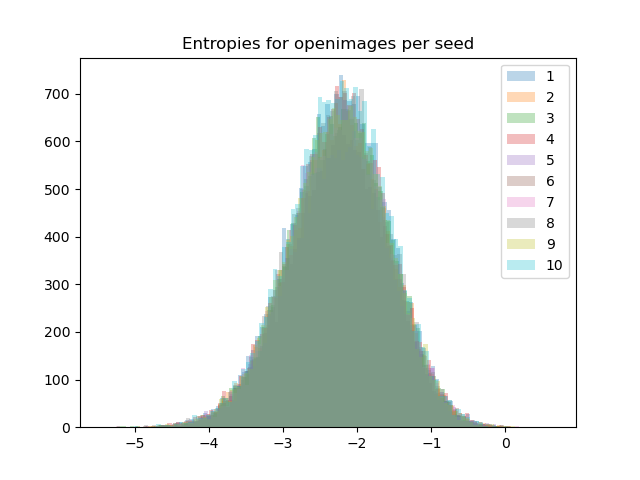
\includegraphics[width=0.9\textwidth]{images/method/probabilistic_independent/openimages_entropies.png}
    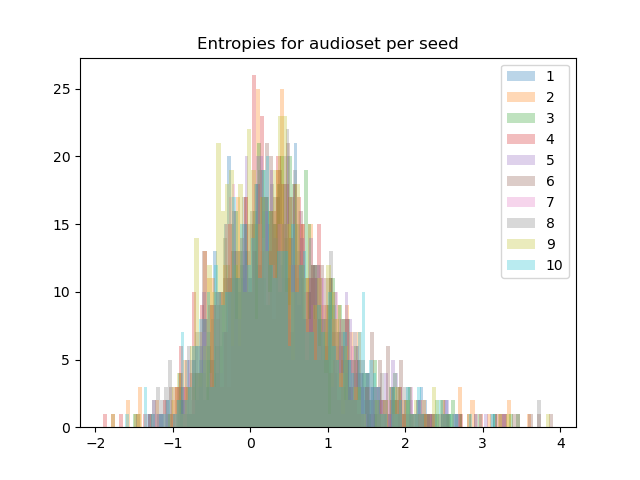
\includegraphics[width=0.9\textwidth]{images/method/probabilistic_independent/audioset_entropies.png}
    \caption{
        Histograms of entropy distributions for Open Images and AudioSet embeddings. 
    }
    % generated by analyse.py 
\end{figure}
 
The histograms indicate that the distributions of the variances of learned embeddings are stable even if the random seed is changed. The AudioSet graph is less smooth because there are only 526 concepts vs. 19996 in Open Images. 
 
We expect that concepts with lower incidence (that are present fewer times in the universe of images / audio clips) should have a higher variance, and therefore higher entropy. This is confirmed by calculating the Spearman correlation of the entropies with the number of incidences of a concept. For AudioSet, this results in a mean Spearman correlation of -0.3465 over 10 random seeds, and for Open Images this is a mean of -0.3369 over 10 random seeds. 

\todo[inline]{We also have the correlation with the deterministic embeddings. Does it mean anything? }

\todo[inline]{Run stability calculation eg. how many of 5-nearest neighbour are present in different runs of same seed, top 200 concepts. }
% audioset
%In [8]: det_learnt_corr.mean()
%Out[8]: 0.9189375433154889
%
%In [9]: entropy_count_rcorr.mean()
%Out[9]: 
%spearmanr   -3.465071e-01
%p            7.865913e-14
%dtype: float64


% openimages
%In [5]: det_learnt_corr.mean()
%Out[5]: 0.2926545426484884
%In [6]: entropy_count_rcorr.mean()
%Out[6]: 
%spearmanr   -0.336871
%p            0.000000
%dtype: float64


% For the following, run inspect_results.py and call mostalike to dump top 5 neighbours for a few seeds
% then 

The table below shows the 3 nearest neighbours (in the rows) to the concept ``Cat" in the Open Images domain, over five seeds. The distance metric is Euclidean distance. There is a consistency to the items, but they do not appear to be very related to the concept of ``Cat".  

    \begin{table}[]
    \begin{tabular}{@{}llll@{}}
Rank / Seed &1 &2 &3 \\
\toprule
1&\begin{tabular}[c]{@{}l@{}} Rope \\ 0.290 \end{tabular}&\begin{tabular}[c]{@{}l@{}} Cage \\ 0.257 \end{tabular}&\begin{tabular}[c]{@{}l@{}} Totem pole \\ 0.392 \end{tabular} \\
2&\begin{tabular}[c]{@{}l@{}} Surfing \\ 0.302 \end{tabular}&\begin{tabular}[c]{@{}l@{}} Human \\ 0.306 \end{tabular}&\begin{tabular}[c]{@{}l@{}} Sketch \\ 0.422 \end{tabular} \\
3&\begin{tabular}[c]{@{}l@{}} Hammock \\ 0.302 \end{tabular}&\begin{tabular}[c]{@{}l@{}} Mammal \\ 0.403 \end{tabular}&\begin{tabular}[c]{@{}l@{}} Peace symbols \\ 0.429 \end{tabular} \\
4&\begin{tabular}[c]{@{}l@{}} Picnic table \\ 0.364 \end{tabular}&\begin{tabular}[c]{@{}l@{}} Fawn \\ 0.412 \end{tabular}&\begin{tabular}[c]{@{}l@{}} Beach \\ 0.429 \end{tabular} \\
5&\begin{tabular}[c]{@{}l@{}} Screenshot \\ 0.394 \end{tabular}&\begin{tabular}[c]{@{}l@{}} Vertebrate \\ 0.421 \end{tabular}&\begin{tabular}[c]{@{}l@{}} Outdoor furniture \\ 0.438 \end{tabular} \\

    \end{tabular}
    \end{table}



This table shows the 5 nearest neighbours to the concept ``Domestic short-haired cat" in the Open Images domain, also over 3 seeds. This looks a lot more sensible. 


    \begin{table}[]
    \begin{tabular}{@{}llll@{}}
Rank / Seed &1 &2 &3 \\
\toprule
1&\begin{tabular}[c]{@{}l@{}} Malayan cat \\ 0.100 \end{tabular}&\begin{tabular}[c]{@{}l@{}} Malayan cat \\ 0.083 \end{tabular}&\begin{tabular}[c]{@{}l@{}} Malayan cat \\ 0.144 \end{tabular} \\
2&\begin{tabular}[c]{@{}l@{}} Burmese \\ 0.195 \end{tabular}&\begin{tabular}[c]{@{}l@{}} Russian blue \\ 0.118 \end{tabular}&\begin{tabular}[c]{@{}l@{}} Himalayan \\ 0.183 \end{tabular} \\
3&\begin{tabular}[c]{@{}l@{}} Russian blue \\ 0.215 \end{tabular}&\begin{tabular}[c]{@{}l@{}} Bombay \\ 0.229 \end{tabular}&\begin{tabular}[c]{@{}l@{}} Russian blue \\ 0.200 \end{tabular} \\
4&\begin{tabular}[c]{@{}l@{}} Abyssinian \\ 0.228 \end{tabular}&\begin{tabular}[c]{@{}l@{}} Polydactyl cat \\ 0.237 \end{tabular}&\begin{tabular}[c]{@{}l@{}} Bengal \\ 0.238 \end{tabular} \\
5&\begin{tabular}[c]{@{}l@{}} Tabby cat \\ 0.240 \end{tabular}&\begin{tabular}[c]{@{}l@{}} Ragdoll \\ 0.256 \end{tabular}&\begin{tabular}[c]{@{}l@{}} Tabby cat \\ 0.267 \end{tabular} \\

    \end{tabular}
    \end{table}


\todo[inline]{It is a known weakness of Euclidean embeddings to represent hierarchical concepts. Hyperbolic / Poincare embeddings may be needed. }


We observe that often, the most specific terms in the domain have more sensible nearest neighbours. For example, these are the 5 nearest neighbours to the concept ``Roti canai", which is a very specific type of Malaysian flatbread. The nearest neighbours are extremely specific and accurate; ``Roti prata", ``Paratha" and ``Uttapam" are all types of Asian flatbread. 

    \begin{table}[]
    \begin{tabular}{@{}llll@{}}
Rank / Seed &1 &2 &3 \\
\toprule
1&\begin{tabular}[c]{@{}l@{}} Roti prata \\ 0.222 \end{tabular}&\begin{tabular}[c]{@{}l@{}} Roti prata \\ 0.264 \end{tabular}&\begin{tabular}[c]{@{}l@{}} Roti prata \\ 0.145 \end{tabular} \\
2&\begin{tabular}[c]{@{}l@{}} Tortilla de patatas \\ 0.235 \end{tabular}&\begin{tabular}[c]{@{}l@{}} Roti \\ 0.299 \end{tabular}&\begin{tabular}[c]{@{}l@{}} Pastelón \\ 0.329 \end{tabular} \\
3&\begin{tabular}[c]{@{}l@{}} Pastelón \\ 0.244 \end{tabular}&\begin{tabular}[c]{@{}l@{}} Paratha \\ 0.303 \end{tabular}&\begin{tabular}[c]{@{}l@{}} Timballo \\ 0.340 \end{tabular} \\
4&\begin{tabular}[c]{@{}l@{}} Paratha \\ 0.287 \end{tabular}&\begin{tabular}[c]{@{}l@{}} Uttapam \\ 0.315 \end{tabular}&\begin{tabular}[c]{@{}l@{}} Pastitsio \\ 0.350 \end{tabular} \\
5&\begin{tabular}[c]{@{}l@{}} Timballo \\ 0.360 \end{tabular}&\begin{tabular}[c]{@{}l@{}} Naan \\ 0.358 \end{tabular}&\begin{tabular}[c]{@{}l@{}} Bobotie \\ 0.376 \end{tabular} \\

    \end{tabular}
    \end{table}



\section{Alignment techniques}

\subsection{Definition of alignment for this problem}

As stated in \cite{ManifoldLearningTheoryAndApplications}, the alignment problem involves finding a transformation of one dataset that maps it to another. 

For this problem, the $x$- and $y$-embeddings (Open Images and AudioSet respectively) are considered to be aligned if the following holds:

\begin{itemize}
    \item For every member of the set $x_{intersect} = y_{intersect}$ of concepts that exist in both domains, the nearest neighbour of mapped concept $f(x_i)$ is the corresponding member $y_i$ in set $y_{intersect}$, and the nearest neighbour of mapped concept $g(y_i)$ is the corresponding member $x_i$ in set $x_{intersect}$. 
\end{itemize}

The accuracy is computed after each epoch of training. It is defined as the fraction of concepts (only in the intersection set) in a domain whose nearest neighbour after mapping is the known other embedding in that domain. 

\subsection{Alignment network}

The alignment network comprises the following:

\begin{itemize}
    \item A probabilistic GloVe embedding layer representing the first domain of embeddings to be aligned (henceforth referred to as the x-embeddings). In the case of these experiments, this is Open Images. 
    \item A probabilistic GloVe embedding layer representing the second domain of embeddings to be aligned (henceforth referred to as the y-embeddings). In the case of these experiments, this is AudioSet. 
    \item A multi-layer perceptron with 3 hidden layers of 100 nodes each, that learns a mapping from the x-embeddings to the y-embeddings: $f(x) \rightarrow y$
    \item A multi-layer perceptron with 3 hidden layers of 100 nodes each, that learns a mapping from the y-embeddings to the x-embeddings: $g(y) \rightarrow x$
\end{itemize}

\todo[inline]{DIAGRAM}

\subsubsection{Full loss function}


The full loss function is

\begin{equation}
\label{eq:fulllossfunction}
\begin{split}
L & = L_{glove, x} + L_{glove, y} + L_{cycle, x} + L_{cycle, y} \\
  & + L_{distance, x-intersect} + L_{distance, y-intersect} \\
  & + L_{distsim, x-intersect} + L_{distsim, y-intersect}
\end{split}
\end{equation}

where the individual components are: 

\begin{itemize}
    \item $L_{glove, x}$: The GloVe loss for $x$ as in \ref{eq:gloveloss}. 
    \item $L_{glove, y}$: The GloVe loss for $y$ as in \ref{eq:gloveloss}. 
    \item $L_{cycle, x}$: The cycle consistency loss from x to y: $||g(f(x)) - y||_2$
    \item $L_{cycle, y}$: The cycle consistency loss from y to x: $||f(g(y)) - x||_2$
    \item $L_{distance, x-intersect}$: The distance loss between $f(x)$ and $y$, for only the intersection of concepts: $||f(x_{intersect}) - y_{intersect}||_2$
    \item $L_{distance, y-intersect}$: The difference between $g(y)$ and $x$, for only the intersection of concepts: $||g(y_{intersect}) - x_{intersect}||_2$
    \item $L_{distsim, x-intersect}$: An optional distributional similarity measure between $f(x_{intersect})$ and $y_{intersect}$
    \item $L_{distsim, y-intersect}$: An optional distributional similarity measure between $g(y_{intersect})$ and $x_{intersect}$
\end{itemize}

and $x_{intersect}$ and $y_{intersect}$ represent the embeddings in both domains of the intersection of concepts between those domains. 

\subsubsection{Other model parameters}

\begin{itemize}
    \item Mini-batch size 500
    \item 10 samples of each concept embedding are taken for each mini-batch for a total of 5000 points per mini-batch
    \item Alignment accuracy is defined as: for $x$, the number of $i$ such that nearest neighbour of $f(x_i)$ is  $y_i$. For $y$, the number of $i$ such that the nearest neighbour of $g(y_i)$ is $x_i$. 
    \item The model is run for 150 epochs; the mean accuracy (over $x$ and $y$) is measured after every epoch and the model is saved if the mean accuracy is greater than the last epoch mean accuracy.
    \item The Adam optimiser is used with a learning rate of 0.01.
    \item No hyperparameter tuning is done. 
\end{itemize}

In the next sections, the individual items in the loss are discussed more thoroughly.

\subsection{GloVe loss}

The GloVe loss equation is restated here:

\begin{equation}
\begin{split}
L_{glove} &= \sum_i \sum_j f(X_{ij}) (\vecw_i^T \vecw_j + b_i + b_j - \log X_{ij})^2\\
f(x) &= \begin{cases}
(x/x_{max})^{\alpha}\spaced{if} x \le x_{max}\\
1\spaced{otherwise}
\end{cases}
\end{split}
\end{equation}

This is a weighted least-squares problem whose solution should be the set of embeddings where each pair $\vecw_i$, $\vecw_j$ should approximate the co-occurrence statistics $X_{ij}$. 

Experimentally, it was found that the GloVe loss had to be scaled by the ratio of concepts: there are 19996 Open Images concepts and 526 Audioset concepts, so the $x$ glove loss (Open Images) is multiplied by 19996 / 526. Without this, the GloVe loss was not enough to result in sensible clusters. 

\subsection{Cycle consistency}

We relate a domain's mapped embeddings (through the $f(x)$ and $g(y)$ MLP layers) to the other domain using what is referred to as cycle-consistency loss. This uses transitivity to self-supervise training; we want $g(f(x))$ to be close to $x$ and $f(g(y))$ to be close to $y$. 

In \cite{CycleGAN}, the reason for requiring cycle consistency is stated: Simply requiring $f(x)$ to be close to $y$ and $g(y)$ to be close to $x$ is insufficient as overfitting can result in a network being able to map an arbitrary set of inputs to an arbitrary set of outputs. In \cite{CycleGAN}, the L1 norm is used, in this experiment we use the L2 norm as we do not want a sparsity constraint imposed on the embeddings. 

Thus the cycle consistency loss takes the following form:

\begin{equation}
\begin{split}
L_{cycle} &= E_x ||f(g(x)) - x||_2 + E_y ||g(f(y) - y||_2
\end{split}
\end{equation}

The analogous equation for $L_{cycle, y}$ has the $x-$ and $y-$ items switched. 

This loss is also used in other alignment architectures, for example \cite{magan} (in which it is known as the reconstruction loss). 

\subsection{Distance loss}

This measures how far away the mapped embedding is from the original embedding. This loss represents the semi-supervised component of the algorithm; it is only calculated for items in the intersection of the 2 concept domains (the 230 concepts present in both Open Images and AudioSet, for our problem). 
\begin{equation}
\begin{split}
L_{distance} &= E_x||f(x) - y||_2 + E_y||g(y) - x||_2
\end{split}
\end{equation}

The Manifold Alignment GAN (MAGAN \cite{magan}) used this loss to guard against the generators (the mapping MLPs in our model) learning a mapping that simply superimposed the manifolds without actually aligning the points, though they use a different formulation for this loss. 

\subsection{Distributional similarity measure}

We would like the distribution of $f(x)$ to be similar to the distribution of $y$, and that of $g(y)$ to be similar to that of $x$. For the intersection of concepts, this means that the distribution of $f(x_{intersect})$ should be similar to $y_{intersect}$, and the distribution of $g(y_{intersect})$ should be similar to $x_{intersect}$. There exist various measures by which two distributions can be compared; for these to be used as loss functions for neural network training, they should generate a scalar value that is minimised when the distributions are identical. 

\subsubsection{Maximum mean discrepancy}

The maximum mean discrepancy (MMD) statistic is introduced in \cite{MMDGretton} as a difference in feature means of the two distributions, where the features are obtained by applying a kernel function to the two samples. Under certain conditions met by the kernel function, the MMD between samples of 2 distributions is 0 if the distributions are identical. Summarising the full theory that can be found in \cite{MMDGretton}, the following conditions must hold:

\begin{itemize}
    \item The kernel must be a characteristic kernel: If the inputs are random variables $X$ with domain $\Omega$ and distribution $P$, there is a one to one mapping between the mean value in feature space and the distributions. \cite{KernelMeanEmbeddingReview} 
    \item That is, each value for the mean in feature space maps to a different possible distribution. 
    \item An intuitive way of looking at this is that the kernel function must be "rich enough" to represent all possible distributions. A known characteristic kernel function that is commonly used is the Gaussian kernel function $k(\vecx, \vecy) = \exp(-\alpha ||\vecx - \vecy||_2^2)$, and this is what we use in our experiments. 
    \item $\alpha$ of 0.01 was used for both domains. This value was chosen because it is close to $\frac{1}{2 \sigma^2}$ where $\sigma$ is the median of the pairwise distances, which is a good heuristic for convergence \cite{Garreau2017LargeSA} . 
\end{itemize}

Given the following:

\begin{itemize}
    \item $\vecx_i$ are $m$ samples from one distribution  $X$
    \item $\vecy_j$ are $n$ samples from the other distribution $Y$
    \item $k(\vecx, \vecx')$ is a characteristic kernel function
\end{itemize}

The empirical unbiased MMD statistic is as follows:

\begin{equation}
\label{eq:mmd}
\begin{split}
MMD (k, x, y) &= \frac{1}{m(m-1)} \sumim \sum_{j \neq i}^m k(\vecx_i, \vecx_j) + \frac{1}{n(n-1)} \sumin \sum_{j \neq i}^n k(\vecy_i, \vecy_j) \\
&- \frac{2}{mn} \sumim \sumjn k(\vecx_i, \vecy_j)
\end{split}
\end{equation}

It can be seen that this is the sum of the within-distribution similarities, less the sum of the cross-distributional similarities. 

%(Can include more items described in http://ssa.cf.ac.uk/big-data/slides/Gretton-MMD-TrainingNetworks.pdf)

The implementation from the \texttt{torch-two-sample} \footnote{\texttt{https://torch-two-sample.readthedocs.io}} library \cite{torchtwosample} was used.  


